\documentclass{standalone}
\usepackage{tikz}

\usepackage{color}

\usetikzlibrary{arrows.meta}
\usetikzlibrary{calc}
\usetikzlibrary{shapes}
\usetikzlibrary{bending}
\usetikzlibrary{patterns}

\usepackage{gensymb}

\usepackage{pgfplots}
\usepackage{amsmath}


\begin{document}
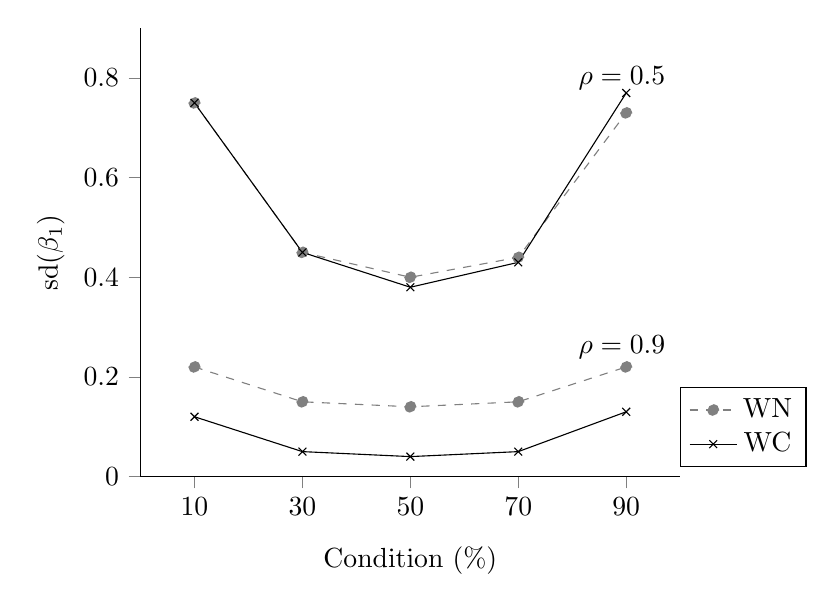
\begin{tikzpicture}[
	%scale=0.4,
	]	
	
	%WN sds
	\begin{axis}[
	axis on top=true,
	%xshift= 6cm,
	scale=1,
	axis x line*=middle , axis y line*=left,
	xtick=\empty,
	%ytick=\empty,
	%extra y ticks = {0.6},
	%extra y tick labels = {$d$},
	ytick align = outside,
	xtick align = outside,
	xlabel = Condition (\%),
	ylabel = sd($\beta_1$),
	extra x ticks = {10,30,50,70,90},
	%extra x ticks = {0.0,1.67},
	%extra x tick labels = {$x_0$,$x_{5}$},
	xlabel near ticks,
	ymin=0, ymax=0.9,
	xmin=0, xmax=100,
	legend style ={at={(1,0.2)}, 
		anchor=north west, draw=black, 
		fill=white}]
	
%	\addplot[mark=*, color=blue]   coordinates {(10,1.74)(30,1.52)(50,1.46)(70,1.5)(90,1.7)};  %rho=0.1
%	\addlegendentry{WN};
%	\addplot[mark=x, color=red]   coordinates{(10,1.8)(30,1.6)(50,1.57)(70,1.6)(90,1.8)} node[pos=0.98] (rho) {};
%	\node [above] at (rho) {$\rho=0.1$}; %rho=0.1
%	\addlegendentry{WC};
	
	\addplot[mark=*, color=gray, dashed]   coordinates {(10,0.75)(30,0.45)(50,0.40)(70,0.44)(90,0.73)};%rho=0.5
	\addlegendentry{WN};
	\addplot[mark=x, color=black]   coordinates {(10,0.75)(30,0.45)(50,0.38)(70,0.43)(90,0.77)} node[pos=0.99] (rho) {};%rho=0.5
	\node [above] at (rho) {$\rho=0.5$};
	\addlegendentry{WC};
	
	\addplot[mark=*, color=gray, dashed]   coordinates {(10,0.22)(30,0.15)(50,0.14)(70,0.15)(90,0.22)} node[pos=0.99] (rho) {}; %rho=0.9
	\node [above] at (rho) {$\rho=0.9$};
	\addplot[mark=x, color=black]   coordinates {(10,0.12)(30,0.05)(50,0.04)(70,0.05)(90,0.13)};%rho=0.9
	
	
	\end{axis}
	
%	%WC sds
%	\begin{axis}[
%	axis on top=true,
%	xshift= 6cm,
%	scale=0.65,
%	axis x line*=middle , axis y line*=left,
%	xtick=\empty,
%	%ytick=\empty,
%	%extra y ticks = {0.6},
%	%extra y tick labels = {$d$},
%	ytick align = outside,
%	xtick align = outside,
%	xlabel = Condition (\%),
%	ylabel = sd($\beta_1$),
%	extra x ticks = {10,30,50,70,90},
%	%extra x ticks = {0.0,1.67},
%	%extra x tick labels = {$x_0$,$x_{5}$},
%	xlabel near ticks,
%	%ymin=0, ymax=1.5,
%	xmin=0, xmax=100]
%
%		\addplot coordinates {(10,1.8)(30,1.6)(50,1.57)(70,1.6)(90,1.8)};
%		
%		\addplot coordinates {(10,0.75)(30,0.45)(50,0.38)(70,0.43)(90,0.77)};
%		
%		\addplot coordinates {(10,0)(30,0.05)(50,0.04)(70,0.05)(90,0.13)};
%
%	\end{axis}

	

	
	
	\end{tikzpicture}  
\end{document}